\subsubsection{整体硬件框图}
%硬件各模块的连接框图（visio）、标注通信标准、融合电源树说明。
\begin{figure}[hbt!]
    \centering
    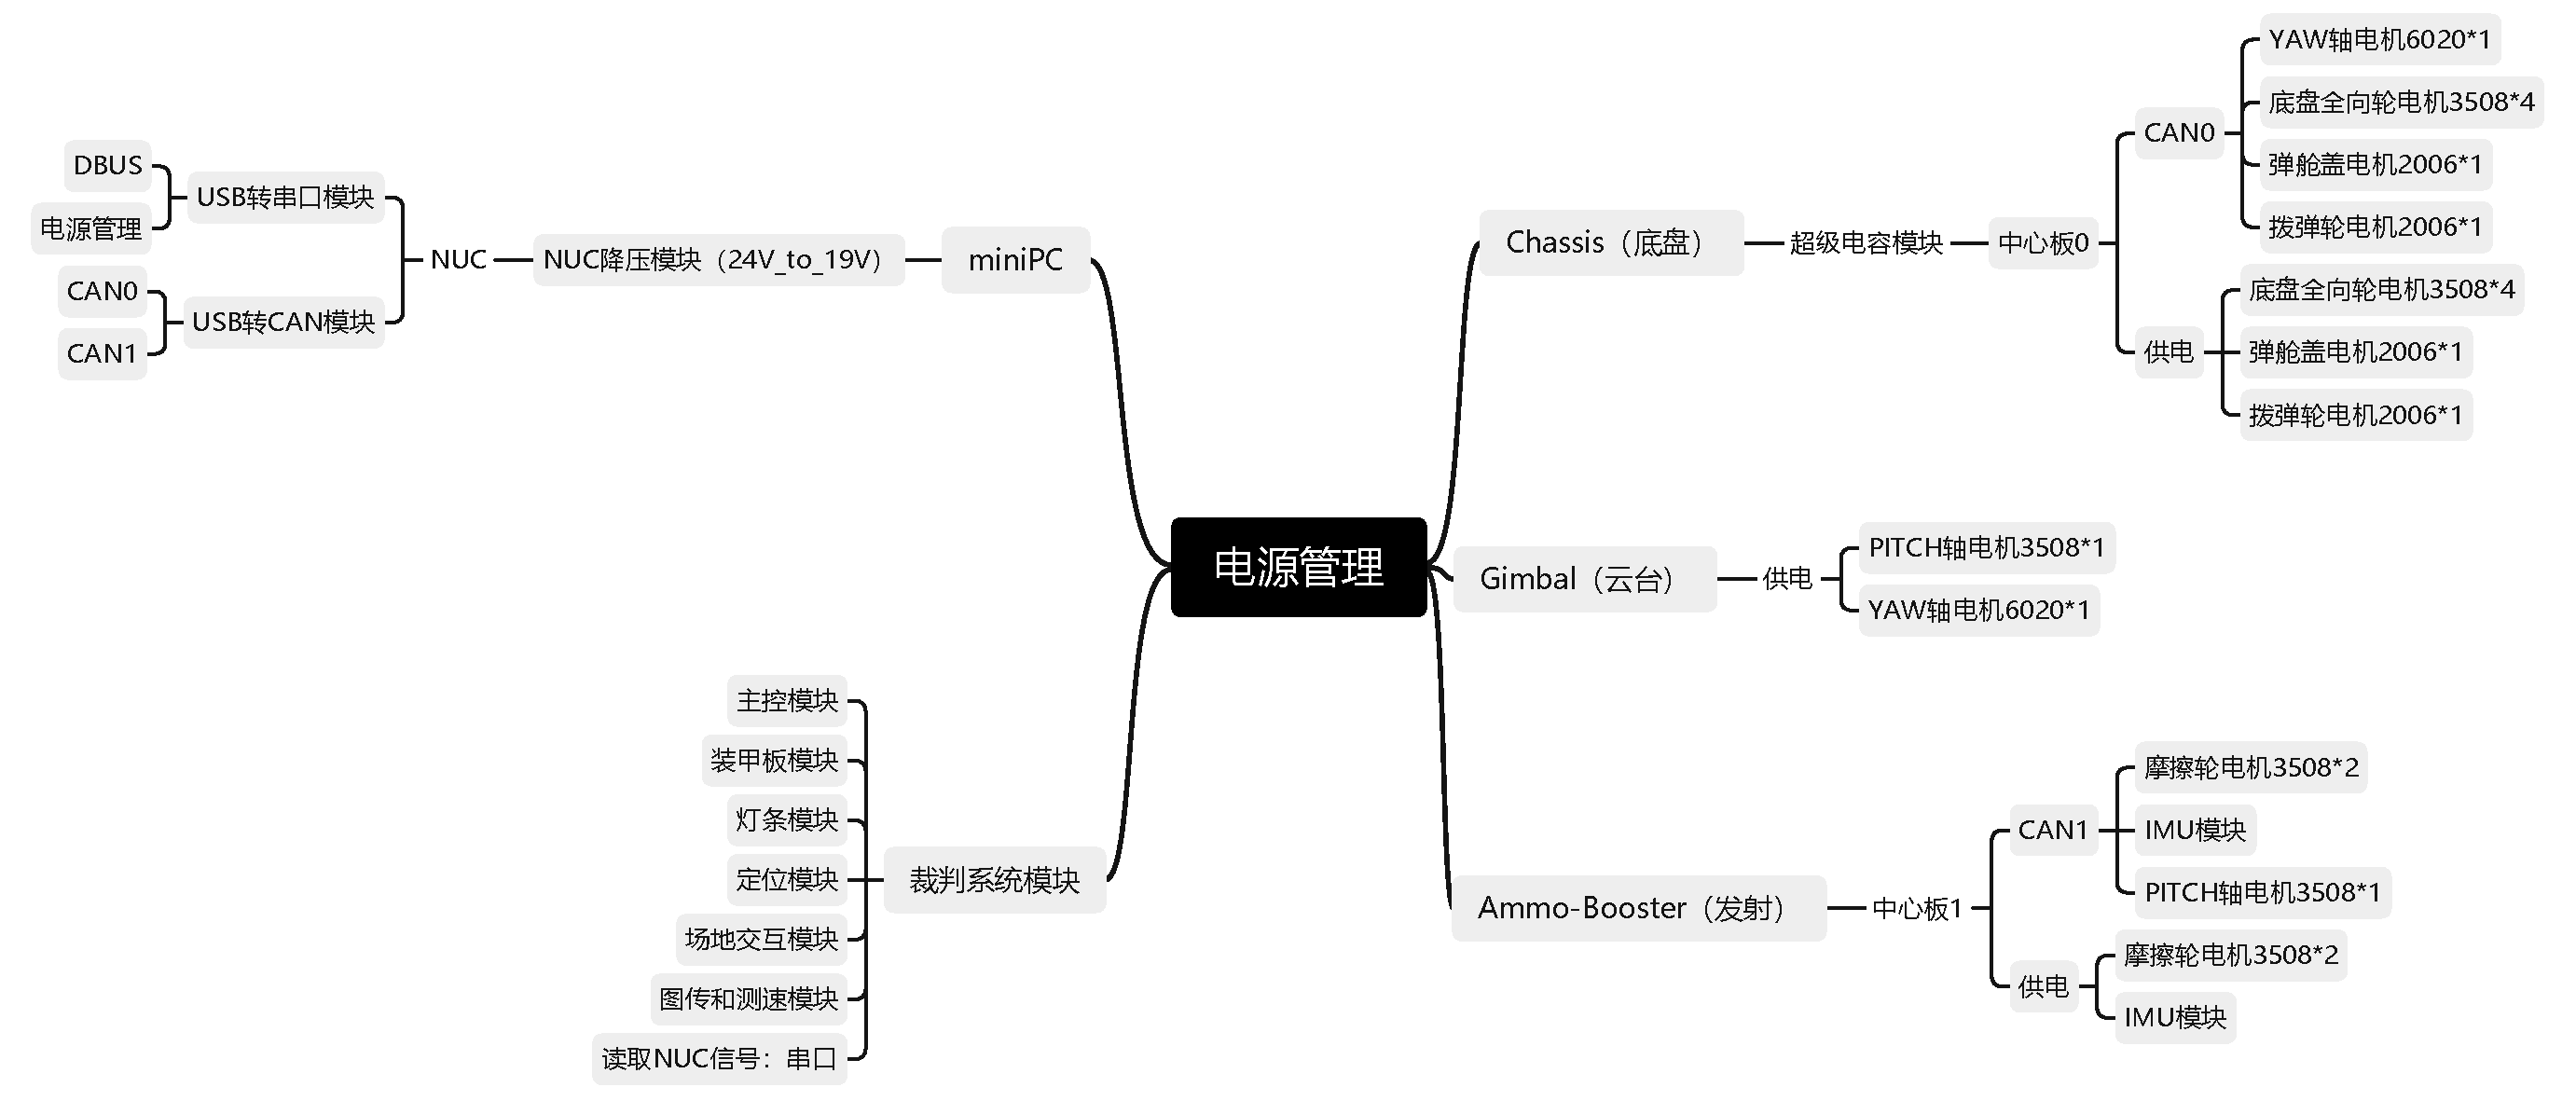
\includegraphics[width=1\columnwidth]{figure/设计方案/硬件设计/hardware_wiring.pdf}
    \caption{整体硬件框图}        
    \label{fig:hardware_wiring_设计方案}
\end{figure}

 \figref {fig:hardware_wiring_设计方案}由电源管理模块出发，从通信和供电两方面介绍了我们步兵机器人的整体硬件电路连接情况。

% \subsection{硬件详细设计（自研）}
%自研电路板功能说明、设计原理图、外设接口等，自研单板有测试报告和记录说明。
\subsection{超级电容}
\begin{figure}[hbt!]
    \centering
    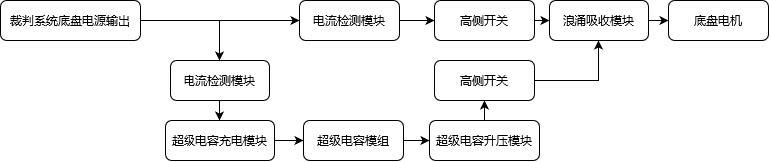
\includegraphics[width=1\columnwidth]{figure/设计方案/硬件设计/超级电容拓扑图.jpg}
    \caption{超级电容拓扑图}        
    \label{fig:super_capacitor_设计方案}
\end{figure}
为了实现超功率模式，我们采用了通用的拓扑结构,如 \figref{fig:super_capacitor_设计方案} 所示。这种拓扑结构的优点是能够容易地实现电容与裁判系统的功率合成以及对拓扑切换时延有一定的容错性。这种结构的主要的功率路径有两个，分别是：
\begin{enumerate}
    \item  经过电流检测模块、高侧开关、浪涌吸收模块后直接提供给底盘电机。
    \item  经过电流检测模块、超级电容充电模块给超级电容模组充电；超级电容经升压模块、高侧开关、浪涌吸收模块后提供给底盘电机。
\end{enumerate}
在装机测试中，在比赛规则限定电池输出功率不超过$\qty{50}{\W}$的条件下，加入了超级电容管理模块之后，可以在保持电池输出功率在$\qty{50}{\W}$时，由电源管理测试模组提供$\qty{120}{\W}$的动力输出长达$\qty{17}{\s}$的时间。

\subsubsection{控制器模块}

控制器模块是超级电容管理模块的计算和控制单元，用于控制其它子模块的工作状态。我们控制器采用意法半导体公司的STM32H750VBT6芯片，该芯片采用Cortex-M7内核，具有六级双发射超标量流水线及分支预测器、单精度及双精度浮点计算单元、紧密耦合内存TCM、高速缓存L1 cache、DSP及MPU单元。我们使其工作在$\qty{480}{\MHz}$的主频下，可以达到约$1207DMIPS$的计算能力。
\par
由于导电滑环的线数不足以再扩展出独立的通信通道，所以微控制器桥接在裁判系统与整车控制器rm-controls中间，通过UART与rm-controls进行通信，桥接后的拓扑结构如\figref{fig:powermanager_bridging_typo} 所示。通信数据包附加在裁判系统数据包后面发出，数据包格式参考中容量数传协议。

\begin{figure}[hbt!]
    \centering
    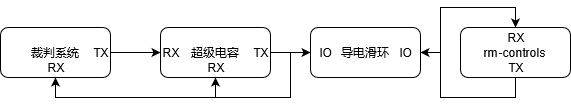
\includegraphics[width=0.8\columnwidth]{figure/设计方案/硬件设计/Topology_Sucap_Bridging.png}
    \caption{桥接后的拓扑结构}
    \label{fig:powermanager_bridging_typo}
\end{figure}

\par
为了实现充电、放电的精准功率监测，我们使用STM32自带的高速16位ADC配合DMA1外设实现对2路电流采样窗口、1路电压采样窗口进行自动循环采样和数据转移。期间还需要配置MPU保护区域、cache禁止缓存区域、ld链接文件等。最终内存空间分配如下：

\begin{figure}[hbt!]
    \centering
    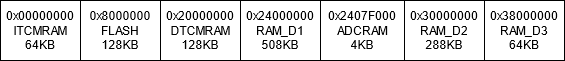
\includegraphics[width=0.8\columnwidth]{figure/设计方案/硬件设计/Sucap_Controller_Memory.png}
    \caption{STM32内存空间分配}
    \label{fig:sucap_controller_memory}
\end{figure}

\par
由于超级电容管理模块是一个模拟、数字、功率器件混合的高系统复杂度的电路系统，并且有诸多的如有限状态机、过流过压欠压保护、裁判系统数据读取转发、功率补偿校正等任务，所以我们使用了开源的FreeRTOS实时操作系统完成系统的调度。为了实现更高的系统实时性，任务调度器被配置到$\qty{10}{\kHz}$的任务切换频率且使用抢占式调度器，并且配置了任务优先级为1的窗口看门狗防止系统卡死在某个状态下。
\par
窗口看门狗很好地预防了系统的卡死，但是在调试的时候看门狗直接复位系统的方法使得卡死时的调试信息无法保存下来，而移植FATFS时FLASH空间不够，所以我们写了一个事件记录器和文件系统。每个事件发生时（如系统掉电、进入超功率模式）就会将事件标志和系统状态记录到文件系统中，后续可以通过回溯信息查找崩溃日志。
\par
在上车调试控制器时，由于车体在运动，无法使用电脑一直连接控制器查看当前的关键系统变量和状态，所以我们写了一个轻量级的GUI界面（Flash占用仅$\qty{8}{\kilo\byte}$），用于绘制电压及功率曲线、任务优先级及堆栈最高水位线、崩溃日志回溯等功能。
\subsubsection{超级电容模组}

电容模组使用$\qty{2.7}{\V}$/$\qty{15}{\F}$电容单体，组合成三并六串的模组，模组标称参数为$\qty{16.2}{\V}$/$\qty{15}{\F}$。如\figref{fig:sucap_single}，由于超级电容单体保护使用阈值为$\qty{2.65}{\V}$的比较器，在单体出现过压时比较器输出高电平控制N-MOS管开启，所以加入了单体保护的超级电容模组可得到新的标称参数$\qty{15.9}{\V}$/$\qty{15}{\F}$，标称容量为$\qty{1896.075}{\J}$。泄放回路为串联式，当单体触发泄放时，总是向下一个单体输出，直到该串中最后的一个电容向GND泄放。这种设计的优点是在单体充电平衡时，并不直接浪费所有能量，可以提高效率；缺点是最后一个泄放MOS管总优先承受最大的泄放电流，直到该串所有的电容电压相等，在使用过程中将使得热量集中于模组的一端，有需要情况下在布局时交叉摆放以减少这种影响。

\begin{figure}[hbt!]
    \centering
    \subfigure[超级电容单体保护电路原理图 \label{fig:sucap_single}]{
        \centering
        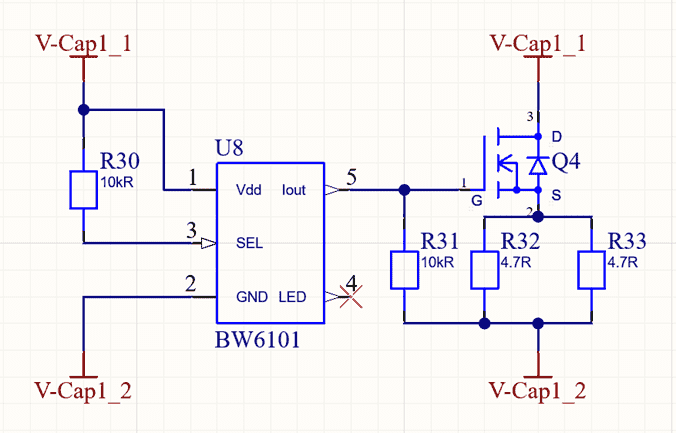
\includegraphics[width=0.48\columnwidth]{figure/设计方案/硬件设计/Sucap_Single.png}
    }
    \subfigure[充电电流采样电路原理图 \label{fig:charge_current_sample}]{
        \centering
        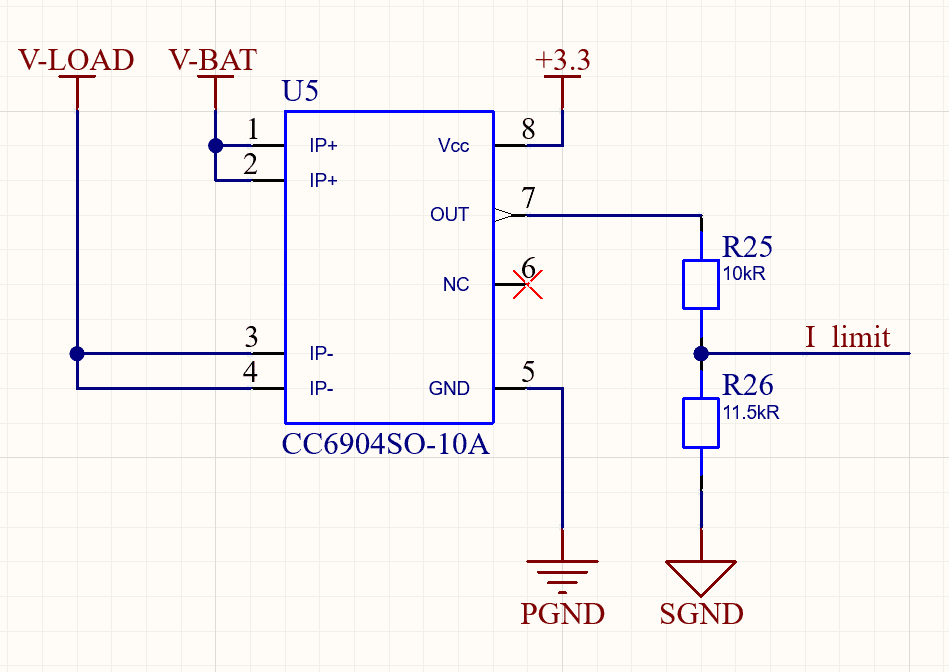
\includegraphics[width=0.44\columnwidth]{figure/设计方案/硬件设计/Charge_Current_Sample.png}
    }
    \caption{部分原理图展示 \label{fig:charge_capacitor_sch}}
\end{figure}
泄放电阻采用两颗2512封装$\qty{4.7}{\Omega}$的电阻堆叠而成，单颗功率耗散为$\qty{2}{\W}$，所以受到泄放电阻的影响，得到该模组总的连续泄放能力为$\qty{53.82}{\W}$，需要加强散热以保证模块的持续稳定工作。
\subsubsection{充电模块}

在充电时，充电模块将负责限制电容的充电功率，且该充电模块可受控于微控制器，连续地控制充电模块的输入电流。本设计中需要控制的是充电电流，在超级电容不同电压下，充电模块恒定输出电流与输入电流差距很大，因此需要微控制器的参与来通过调整输出电流以实现对输入电流（即输入功率）的限制。
\par
充电模块使用了专用的超级电容充电控制器BQ24640，该控制器是TI为超级电容模组充电所设计的一款专用芯片，基本拓扑是同步型Buck，集成了电流差分采样放大器，通过在电源的输出对一个模拟输入端口设置电压并在控制器内部进行比较，从而达到电流限制的目的。由于集成的差分放大器差分输入量程为$0\sim100mV$，在差分输入只有$\qty{5}{\mV}$时，电流控制的误差将达到$\pm25\%$以上。为保证电流控制的精度，这里选用$\qty{10}{\omega}$的采样电阻。根据数据手册公式\eqref{equ:chg_out_current}，可求出输出电流为$I_{charge} = \qty{10}{\A}$。

\begin{equation}
    I_{charge} = \frac{V_{iset}}{K V_{iset-max}\times\qty{100}{\mV}}
    \label{equ:chg_out_current}
\end{equation}

\par
BQ24640电压基准$V_{iset}$的上拉电阻被微控制器的DAC输出上拉，在电压基准未触发时，呈现高阻状态，ISET节点电压与DAC输出电压相等，此时充电模块输出电流受控于微控制器。充电模块的原理图如 \figref  {fig:charge_circuit_schematic} 所示。

\begin{figure}[hbt!]
    \centering
    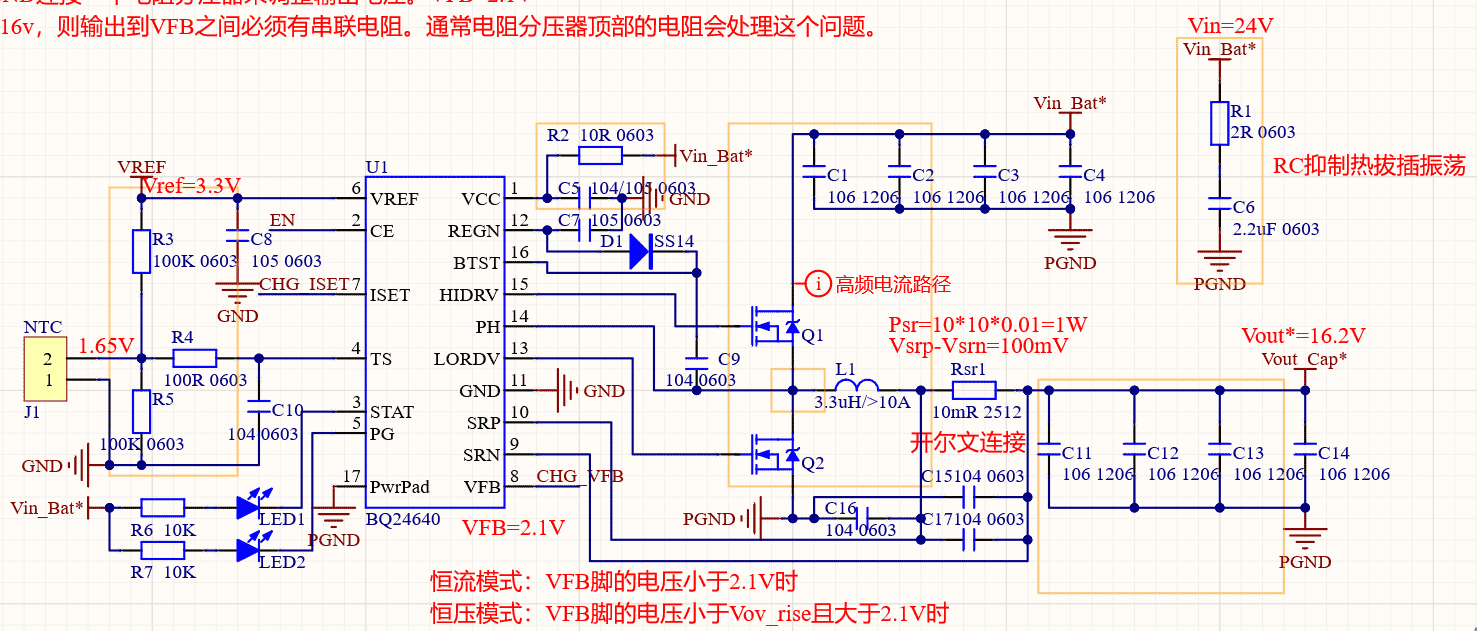
\includegraphics[width=0.8\columnwidth]{figure/设计方案/硬件设计/Charge_Circuit_Schematic.png}
    \caption{充电模块原理图}
    \label{fig:charge_circuit_schematic}
\end{figure}

\subsubsection{高侧开关模块}

高侧开关用于控制上述模块之间的连通性。我们使用了TI的高侧保护控制器LM5060替代了以前使用的BTS443P。如 \figref {fig:high_side_switch_bts443p} 。该高侧保护控制器使用恒流驱动外置的NMOS，我们使用了两颗仅$\qty{5.2}{\m\Omega}$的NMOS HSBA6040实现防浪涌的功能。该高侧保护还具有过压保护、欠压保护、过流保护和故障延时重启等功能。

\begin{figure}[hbt!]
    \centering
    \subfigure[使用BTS443P作为高侧开关 \label{fig:high_side_switch_pmos}]{
        \begin{minipage}[t]{0.45\linewidth}
        \centering
        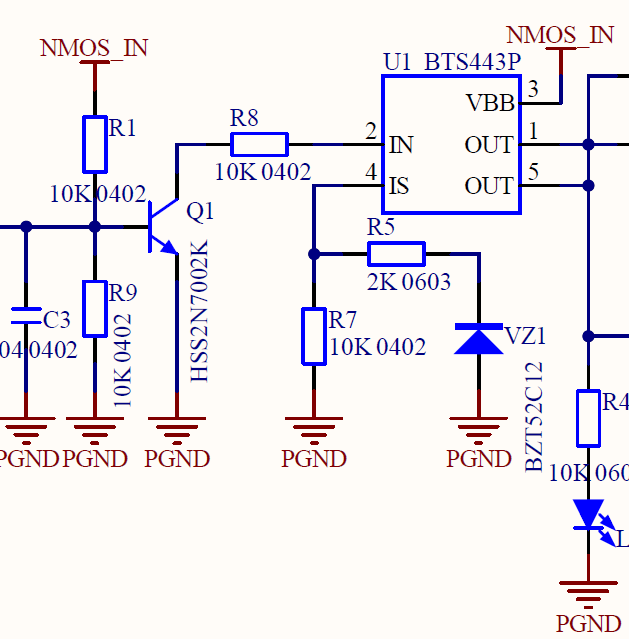
\includegraphics[width=0.7\columnwidth]{figure/设计方案/硬件设计/BTS443P_Switch.png}
        \end{minipage}
    }
    \subfigure[使用BTS443P作为高侧开关 \label{fig:high_side_switch_bts443p}]{
        \begin{minipage}[t]{0.45\linewidth}
        \centering
        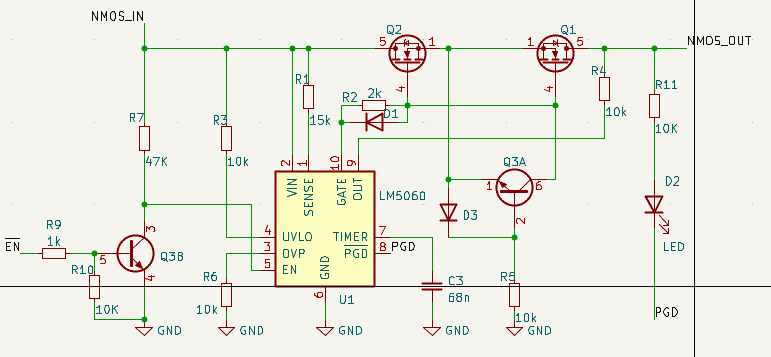
\includegraphics[width=0.7\columnwidth]{figure/设计方案/硬件设计/HighSideSwitch-LM5060.png}
        \end{minipage}
    }
    \caption{高侧开关原理图 \label{fig:high_side_switch_sch}}
\end{figure}

\par
另外，我们还通过三极管实现反相器，将所有的模块（包括高侧开关）使能电平统一设定为低电平。这在微控制器故障或与模块使能引脚连接不稳定使引脚浮空浮空的时候可以避免模块被误开启。

\subsubsection{浪涌吸收模块}
在刚开始的时候，由于我们选择的高侧开关是一颗耐压为$\qty{40}{\V}$的PMOS管。在底盘电机刹车或正反转切换的瞬间高侧开关就会烧毁。所以我们通过示波器测量了单个M3508电机在刹车和正反转切换时的电压跳动情况如 \figref {fig:no_surge_absorbing_brake} 和 \figref {fig:no_surge_absorbing_switch} 所示，最高钳位电压达到了$\qty{50}{\V}$，足以过压击穿PMOS。所以我们先设计了一个利用肖特基二极管和电解电容器作为浪涌吸收的模块如 \figref {fig:surge_absorbing_early}。

\begin{figure}[hbt!]
    \centering
    \subfigure[无浪涌吸收刹车 \label{fig:no_surge_absorbing_brake}]{
        \centering
        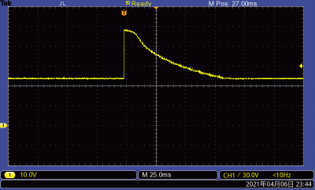
\includegraphics[width=0.23\columnwidth]{figure/设计方案/硬件设计/No_Surge_Absorbing_Brake.png}
    }
    \subfigure[有浪涌吸收刹车 \label{fig:have_surge_absorbing_brake}]{
        \centering
        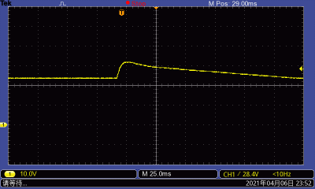
\includegraphics[width=0.23\columnwidth]{figure/设计方案/硬件设计/Have_Surge_Absorbing_Brake.png}
    }
    \subfigure[有浪涌吸收正反切 \label{fig:no_surge_absorbing_switch}]{
        \centering
        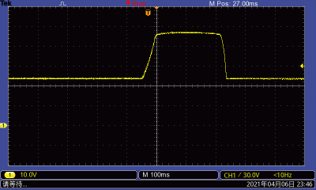
\includegraphics[width=0.23\columnwidth]{figure/设计方案/硬件设计/No_Surge_Absorbing_Switch.png}
    }
    \subfigure[无浪涌吸收正反切 \label{fig:have_surge_absorbing_switch}]{
        \centering
        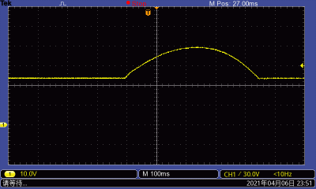
\includegraphics[width=0.23\columnwidth]{figure/设计方案/硬件设计/Have_Surge_Absorbing_Switch.png}
    }
    \caption{有浪涌吸收模块对比 \label{fig:wheather_have_surge_absorbing_compare}}
\end{figure}

\par
在增加了浪涌保护模块后，在浪涌保护模块的输出侧用万用表进行波形的测量。可以看到，有浪涌保护模块的电机刹车电压波形变成了 \figref {fig:have_surge_absorbing_brake}，正反转切换变成了 \figref {fig:have_surge_absorbing_switch}。从图中可以看出，最高电压大概在$\qty{40}{\V}$，且在正反切的图中波形变成了圆滑的圆弧状，说明在切换的过程中电容有能量的储存，在正反转切换的瞬间不会继续从电源获取能量，实现了浪涌吸收和能量回收的效果。

\par
在测试时，发现当负载功率达到$\qty{240}{\W}$时，我们采用的肖特基二极管SVM1550UB的发热严重，需要加装散热片来保证芯片不会烧毁。于是分析负载功率达到$\qty{240}{\W}$时肖特基二极管上的功率耗散，有公式\eqref{equ:diode_power_dissipation}求得$P_{diode}=\qty{4.9}{\W}$，可见损耗率达到了$2.1\%$。所以我们采用了TI公司的LM5050理想二极管控制器，配合CSD18540 MOS管替换掉肖特基二极管。可求得此时的$P_{dis}=\qty{0.22}{\W}$，损耗可以忽略不计
。
\begin{equation}
    P_{diode}=\frac{P_{out}}{24V} U_{diode} = {\frac{P_{out}}{24V}}^2  R_{DS}
    \label{equ:diode_power_dissipation}
\end{equation}

\begin{figure}[hbt!]
    \centering
    \subfigure[早期版本电路 \label{fig:surge_absorbing_early}]{
        \centering
        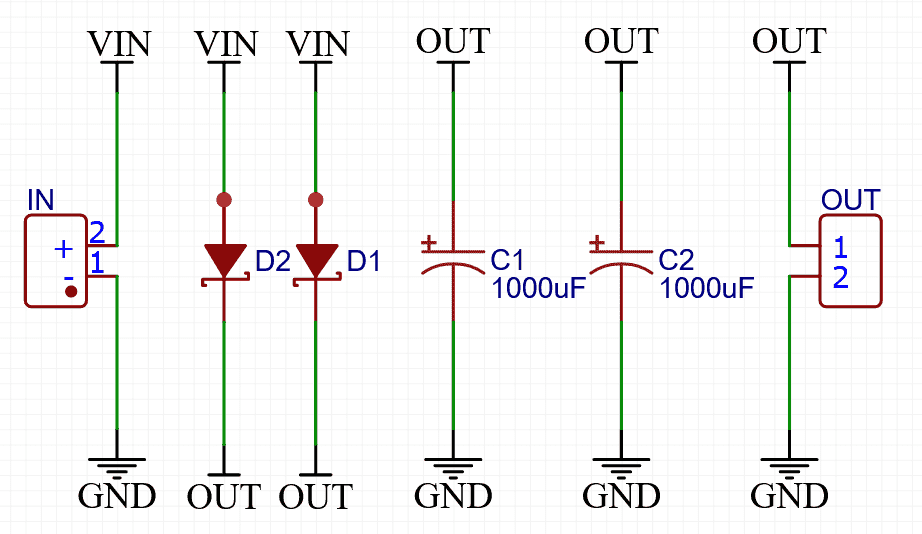
\includegraphics[width=0.4\columnwidth]{figure/设计方案/硬件设计/Surge_Absorbing_Early.png}
    }
    \subfigure[现在版本电路 \label{fig:surge_absorbing_now}]{
        \centering
        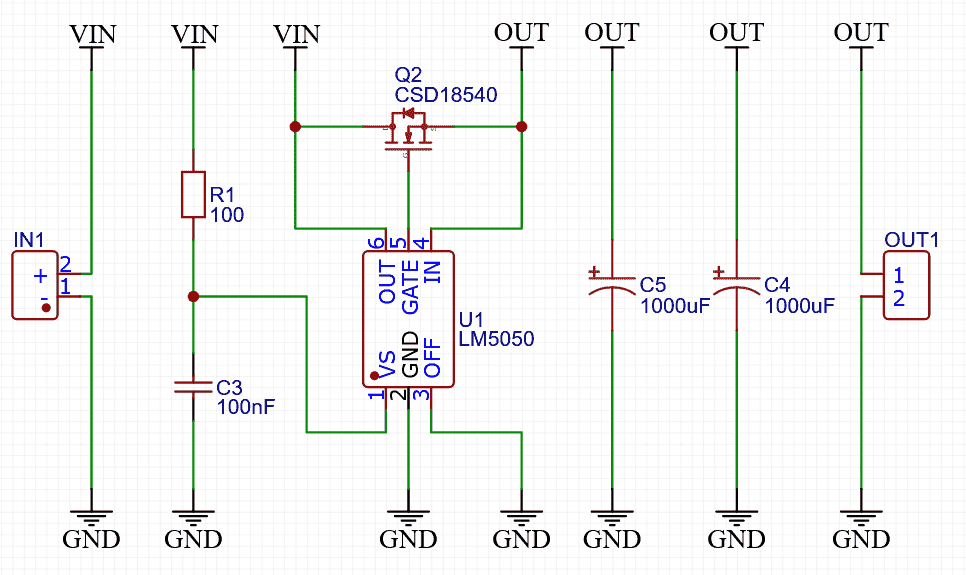
\includegraphics[width=0.4\columnwidth]{figure/设计方案/硬件设计/Surge_Absorbing_Now.png}
    }
    \caption{早期和现在的浪涌吸收模块 \label{fig:surge_absorbing_version}}
\end{figure}

\subsubsection{升压模块}
如 \figref {fig:升压1.0版本大小对比}所示，在超级电容中，升压模块1.0版本的设计最大功率为电源管理额定功率的两倍，即$\qty{240}{\W}$。由于升压模块有最低的输入电压限制，以及在输入输出电压压差较大时会导致输出端产生很大的纹波，且电源转换效率会变得很低，所以我们将升压模块的输入电压范围设置为$7\sim16V$。在1.0版本中采用两相供电技术，其中一相在原有的纹波波谷处补充输出，首先直接补偿了原有的电压跌落，且在同样的频率下，由于两相半桥开关状态相互错开，输出纹波的频率即为开关频率的两倍，更高频的纹波简化了输出滤波的设计，单个电感中的开关电流也会减小，提高功率密度。
\begin{figure}[hbt!]
    \centering
    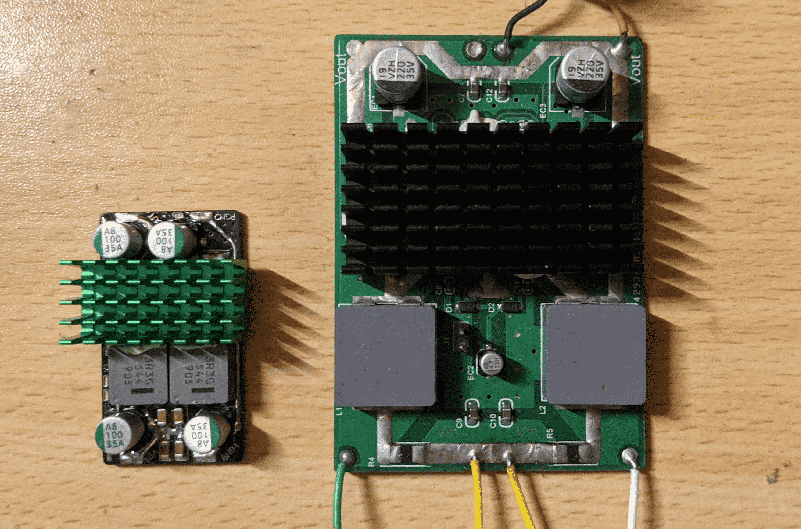
\includegraphics[width=0.6\columnwidth]{figure/设计方案/硬件设计/Boost_Version_Compare.jpg}
    \caption{升压1.0版本大小对比}     
    \label{fig:升压1.0版本大小对比}
\end{figure}

\par
在此我们采用了ADI的多相同步升压控制器LTC3784，单颗控制器可提供两相互补的PWM输出，分别驱动两对半桥，可在较小的输出电容配置时，高输出电流下仍能具有高效率和低输出纹波。为解决多相供电技术的瞬态性能比同步多路并联稍差的问题，LTC3784提供了电流模式的误差放大器反馈环路补偿功能，通过匹配反馈网络的前馈电容和补偿节点的RC网络的器件参数，可以使多相供电的瞬态性能得到十分大的改善。

\par
升压模块2.0版本也采用ADI的多相同步升压控制器，但是型号上我们选取了LTC3897的双片四相方案，如 \figref{fig:四相拓扑连接图}所示，实现$\qty{480}{\W}$（$\qty{24}{\V}$$\qty{20}{\A}$)的超大功率。四相的方案选择让元器件选型、散热变得更加容易，纹波更低的同时也提高了效率。

\begin{figure}[hbt!]
    \centering
    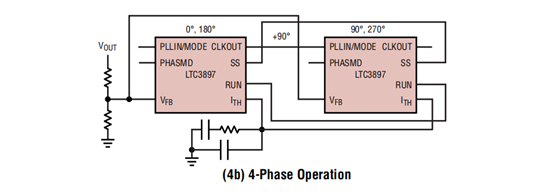
\includegraphics[width=0.9\columnwidth]{figure/设计方案/硬件设计/四相连接图.png}
    \caption{四相拓扑连接图}        
    \label{fig:四相拓扑连接图}
\end{figure}
LTC3897与LTC3784相比,其在宽输入范围的同时，内置了一个理想二极管控制器和浪涌停止器，三个控制器可以单独使用，这让我们得以节省一个输出端的高侧开关模块。单颗LTC3897实现两相PWM互补输出，两个并联通过芯片内部的锁相环实现频率同步，通过PHASMD引脚悬空实现相为$90^{\circ}$互补，让双片四相的方案得以实现。

 \begin{figure}[hbt!]
    \centering
    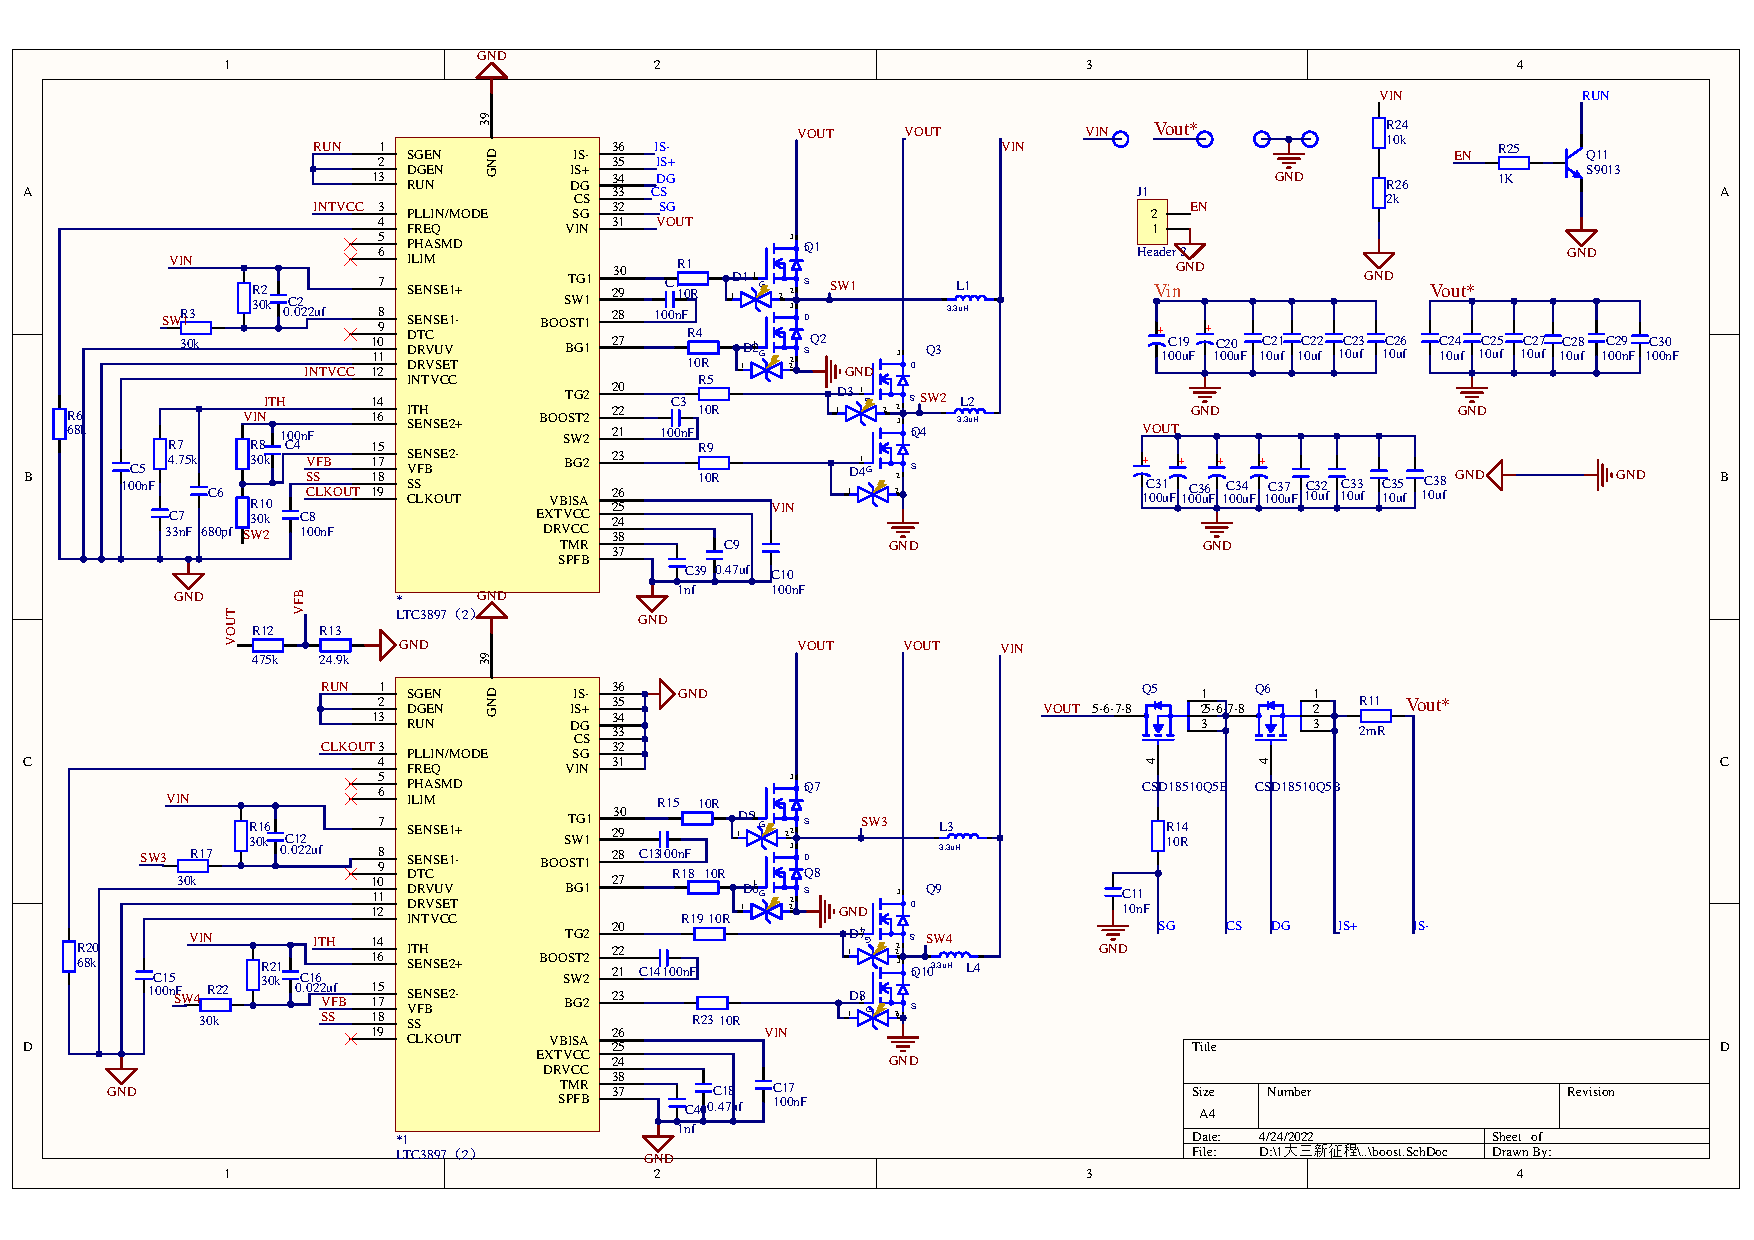
\includegraphics[width=0.7\columnwidth]{figure/设计方案/硬件设计/boost.pdf}
    \caption{升压2.0原理图}        
    \label{fig:升压2.0原理图}
\end{figure}

\subsubsection{升压模块功率器件选型}
\textbf{电感选型}：考虑到板面体积不能太大，这里选用了封装为1054的松下的ETQP5M2R5YFC的电感，标称的感量为$\qty{2.5}{\W}$，在加强散热时额定电流为$\qty{18.1}{\A}$，饱和电流$\qty{27.2}{\A}$，以下将在此基础上进行电压范围和工作频率的确定。根据电感的纹波电流容易列出不等式\eqref{equ:boost_inductance_current}。

\begin{equation}
    \frac{I_{out(max)}\times V_{out}}{2\times V_{in}} + \frac{V_{in}}{2\times f_{SW}\times L}\times (1-\frac{V_{in}}{V_{out}}) < 18.1A
    \label{equ:boost_inductance_current}
\end{equation}

\par
降低频率可以降低MOS管开关损耗，却会增大电感的纹波电流，为提高效率和留有足够的裕量，设定输入电压为$\qty{7}{\V}$，工作频率为$\qty{644}{\kHz}$，此时最大的$\Delta I_L  \approx 0.6I_{max}$，处于较良好的范围内。

\par
\textbf{MOS管选型}：设控制管，即半桥的下管损耗功率为$P_{ctrl}$；同步管，即半桥的上管损耗功率为$P_{sync}$，则有公式\eqref{equ:boost_mosfet_powerloss1}和\eqref{equ:boost_mosfet_powerloss2}：

\begin{equation}
    P_{ctrl} = \frac{(V_{out}-V_{in})V_{out}}{V_{in}^2} (\frac{I_{out(max)}}{2})^2 (1+\delta) R_{DS(ON)} + k \cdot V_{out}^3 \frac{I_{out(max)}}{2 \times V_{in}} \cdot C_{miller} \cdot f
    \label{equ:boost_mosfet_powerloss1}
\end{equation}

\begin{equation}
P_{sync}=\frac{V_{in}}{V_{out}} \times (\frac{I_{out(max)}}{2})^2 \times (1+\delta) \times R_{DS(ON)}
    \label{equ:boost_mosfet_powerloss2}
\end{equation}

\par
将两式中的$(\frac{I_{out(max)}}{2})^2 (1+\sigma)$约去，又$\frac{(V_{out}-V_{in})V_{out}}{V_{in}^2}$可写成$(\frac {V_{out}}{V_{in}})^2-\frac{V_{out}}{V_{in}}$，因为最大输入电压为$\qty{16}{\V}$，输出电压为$\qty{26.4}{\V}$，，可得$(\frac {V_{out}}{V_{in}})^2-\frac{V_{out}}{V_{in}} \geq 1.016$。又$\frac{V_{out}}{V_{in}}<1$。根据手册，k的经验值为$1.7$，易得在本设计中$P_{ctrl}>P_{sync}$，故在控制管选型时，需要注意结温的温升系数，选取导通电阻和米勒电容更小的MOS管。
\par
最终升压模块选用HSBB4052作为同步管，由于该款MOS管的封装使用的是$\qty{16}{\V}$，的无引线扁平封装，在低电压时选用该MOS管作为控制管温升将超过了该款MOS管$\qty{50}{\circ}$，C的最大容许工作温度极限，所以选用了NTMFS5C670NL作为控制管。这两种型号都具有极低的栅极充电电荷和米勒电容，极大地减少了高工作频率下MOS管开关动作引起的损耗。
\begin{figure}[hbt!]
    \centering
    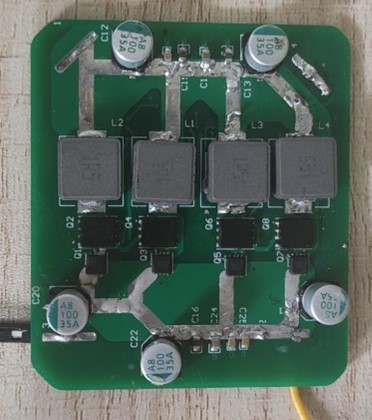
\includegraphics[width=0.26\columnwidth ,angle=90]{figure/设计方案/硬件设计/Boost2.0_test.jpg}
    \caption{升压2.0测试版}        
    \label{fig:升压2.0测试版}
\end{figure}

\subsubsection{环路补偿电路计算}
\textbf{环路补偿}：首先要确定前馈电容和衰减电容的大小，前馈电容$C_{ff}$是一个与反馈网络中$R_{top}$并联的电容，滤波电容$C_{flt}$则是与$R_{bot}$并联的，未添加前馈电容时，反馈网络的增益由分压电阻大小决定，其计算公式如\eqref{equ:boost_dc_gain}。在反馈网络中添加前馈电容后，电源的输出可以更高效地响应高频扰动，但前馈电容可能会引入不想要的开关噪声，因此可添加一个衰减电容用于减小引入前馈电容后的增益，避免高频段增益接近$\qty{0}{\dB}$，时系统不稳定。前馈电容一般在$\qty{1000}{\pF}$，以下，由于电容的阻抗特性，反馈网络的低频区仍与不加前馈电容时一致；而在中高频区域，前馈电容为输出的扰动到反馈端提供了低阻抗通路，促使电源控制器对负载顺便产生更快的响应。添加前馈电容后在反馈网络的零点频率后引入了增益增量，当处于零点和极点频率之间时，该增量的达到最大值。反馈网络的零点$f_z$和极点$f_p$可以由公式\eqref{equ:boost_comp_zero}和\eqref{equ:boost_comp_pole}计算得出。

\begin{equation}
    DC\ gain=20 \cdot lg(\frac{R_{top}}{R_{top}+R_{bot}})
    \label{equ:boost_dc_gain}
\end{equation}

\begin{equation}
    f_z=\frac{1}{2\pi \cdot R_{top} \cdot C_{ff}}
    \label{equ:boost_comp_zero}
\end{equation}

\begin{equation}
    f_p=\frac{1}{2\pi \cdot (C_{ff}+C_{flt})} \cdot (\frac{1}{R_{top}} +\frac{1}{R_{bot}})
    \label{equ:boost_comp_pole}
\end{equation}

\par
由公式可看出零、极点的频率与前馈电容的大小成反比。要获得充足的相位裕度并充分衰减噪声，反馈网络的穿越频率应选为工作频率的1/10至1/6，可得在本设计中该频率范围为$\qty{64.4}{\kHz}\sim\qty{107.3}{\kHz}$。当使零、极点的频率的几何平均值为反馈网络的穿越频率时，可得到最优化的响应，即可列出公式$f_{cross}=\sqrt{f_z \times f_p}$。代入\eqref{equ:boost_comp_zero}和\eqref{equ:boost_comp_pole}有：

\[
f_{cross}=\frac{1}{2\pi} \cdot \sqrt{\frac{1}{C_{ff} \cdot (C_{ff}+C_{flt})} \cdot \frac{1}{R_{top}} \cdot (\frac{1}{R_{top}} +\frac{1}{R_{bot}})}
\]

可画出如 \figref {fig:boost_cff_cfft_range} 曲线，横轴为$C_{ff}$，纵轴为$C_{flt}$，处于两范围交集内的电容值都是可用的，由于零点频率只与$C_{ff}$相关，更大的$C_{ff}$使得零点变得过低，使在低频区域的增益变得过大，系统对噪声过于敏感，所以首先选取靠近左上角的标准电容值，即取$C_{ff}=\qty{180}{\pF}$，$C_{flt}=\qty{910}{\pF}$。
\begin{figure}[hbt!]
    \centering
    \subfigure[$C_{ff}$与$C_{flt}$选择范围 \label{fig:boost_cff_cfft_range}]{
        \centering
        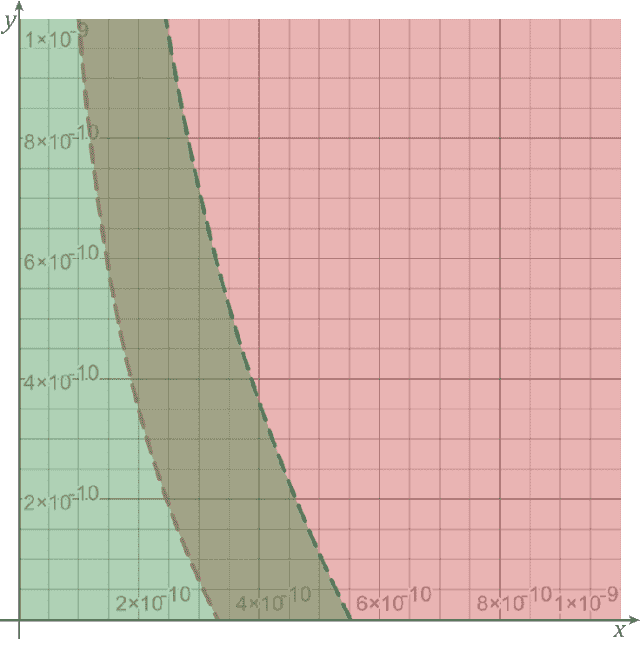
\includegraphics[width=0.44\columnwidth]{figure/设计方案/硬件设计/Boost_Cff_Cfft_Range.png}
    }
    \subfigure[环路带宽限制 \label{fig:boost_bandwidth_limit}]{
        \centering
        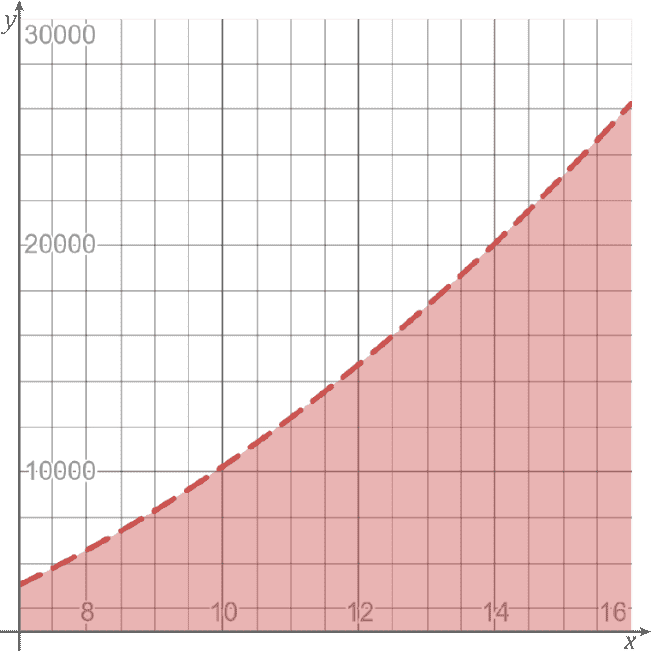
\includegraphics[width=0.44\columnwidth]{figure/设计方案/硬件设计/Boost_Bandwidth_Limit.png}
    }
    \caption{Boost环路补偿计算}
    \label{fig:boost_loop_cal1}
\end{figure}
\par
由于Boost拓扑在连续导通模式下，环路中会出现右半平面零点（RHPZ），使瞬态响应特征变差，这是由于在负载电流变大时，占空比也会变大，在短时间内电感向负载供电的时间变短，电压反而下降得更多，需要几个周期后才能恢复。根据经验，一般的设计要求环路的带宽（或称环路的穿越频率，为避免混淆，以下均称为环路带宽）低于1/3的右半平面零点频率，右半平面零点频率可由公式\eqref{equ:boost_loop_RHPZ_freq}算出。$R_{out}$为负载电阻，$L$为电源选用的功率电感，当电源的输入电压和负载电阻越小，此时右半平面零点频率越低，负载电阻由输出电流直接决定，环路带宽的公式为\eqref{equ:boost_loop_bandwidth}。

\begin{equation}
    f_{rhpz}=\frac{R_{out}}{2\pi \cdot L} \cdot (\frac{V_{in}}{V_{out}})^2
    \label{equ:boost_loop_RHPZ_freq}
\end{equation}

\begin{equation}
    f_{band} < \frac{V_{out}}{6\pi\cdot L \cdot I_{out}} \cdot (\frac{V_{in}}{V_{out}})^2
    \label{equ:boost_loop_bandwidth}
\end{equation}

\par
当电流很小时，带宽即使很高系统也能稳定，所以仅需考虑最大电流时的情况，如 \figref {fig:boost_bandwidth_limit} 为最大电流时环路带宽的限制（横轴x为输入电压$\qty{}{\V}$，纵轴y为带宽频率$\qty{}{\kHz}$）。
\par
确定环路的带宽限制后，现在开始进行II型补偿网络设计，如 \figref {fig:boost_loop_compensation_sch}，由于电流型控制器的跨导型误差放大器输出并非理想电流源，具有一个大内阻$R_0$，由LTC3784的数据手册读取到$R_0=\qty{2}{\m\Omega}$，即可计算出环路的第一个极点，其余的参数由补偿网络的器件数值确定，最后应使得环路响应符合 \figref {fig:boost_type2_compensation_relation} 的要求。为简化计算，这些步骤在LTpowerCAD中完成。

\par
使用可视化的方法可以快速地确定参数，如 \figref {fig:boost_type2_compensation_relation}，调整$C_{TH}$将影响第一极点和零点的位置，更小的$C_{TH}$值将使得增益曲线的第一个下降的斜边向由平移，使得高增益区间向高频拓展，使电源在负载阶跃中更快的达到稳态，但零点频率提高会导致目标带宽处的相位裕度不足；而更大的$R_{TH}$使得增益曲线的中频平台向上平移，且直接增大电源的带宽，使得在负载阶跃时过充和下冲减小，但过高的带宽会令相位裕度变差；更小的$C_{THP}$使第二极点的位置向高频移动，$C_{THP}$作为环路补偿引脚的去耦电容，可降低补偿节点的噪声，但过大的$C_{THP}$使得带宽变小，使电源的瞬态响应变慢，应配置$C_{THP}$使第二极点频率低于工作频率且高于电源的带宽，以较好消除开关噪声的同时保证有足够的相位裕度。
\par
改变输入电压和电流，确保系统的参数能使电源的环路是稳定的同时，在右侧估算的电流阶跃响应有足够好的效果。此处只需关注环路的稳定性即可，对于纹波的仿真将会在下一段得到一个较为理想的结果。

\begin{figure}[hbt!]
    \centering
    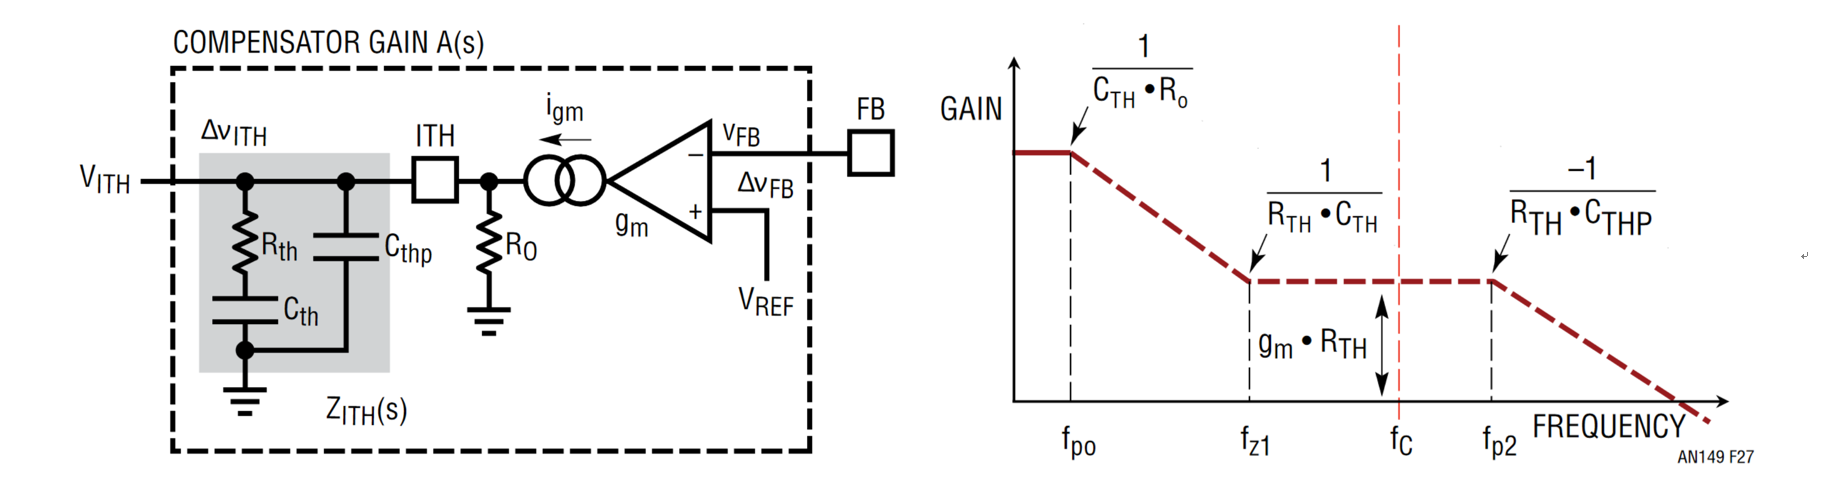
\includegraphics[width=1\columnwidth]{figure/设计方案/硬件设计/Boost_Loop_Compensation_Sch.PNG}
    \caption{环路补偿网络框图与补偿增益曲线}
    \label{fig:boost_loop_compensation_sch}
\end{figure}

\begin{figure}[hbt!]
    \centering
    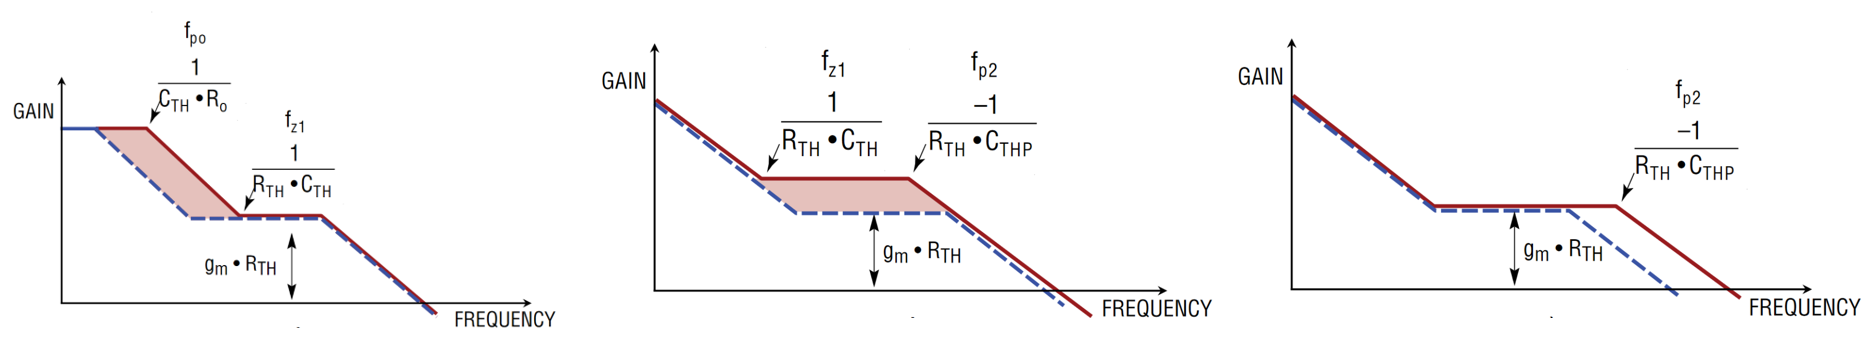
\includegraphics[width=1\columnwidth]{figure/设计方案/硬件设计/Boost_Type2_Compensation_Relation.PNG}
    \caption{II型补偿网络器件参数与补偿增益曲线关系}
    \label{fig:boost_type2_compensation_relation}
\end{figure}


\subsubsection{计算机辅助设计验证仿真}

本模块的设计将使用ADI提供的LTpowerCAD以及LTspice等工具进行辅助设计和仿真。如 \figref{fig:ltpowercad_power_stage} 所示，首先使用LTpowerCAD辅助确定包括环路补偿在内的参数。确定参数后，使用LTspice仿真电源的运行效果。如 \figref {fig:ltspice_simulation} 所示，搭建原理图，设置输入电压为$\qty{13.8}{\V}$，仿真电感纹波电流最大的状况，以确定最大的输出纹波电压。仿真得纹波电压为$\qty{0.031}{\V}$，纹波系数仅有$1.12\textperthousand$。至此，升压模块设计告一段落。

\begin{figure}[hbt!]
    \centering
    \subfigure[LTpowerCAD功率级设计页面 \label{fig:ltpowercad_power_stage}]{
        \centering
        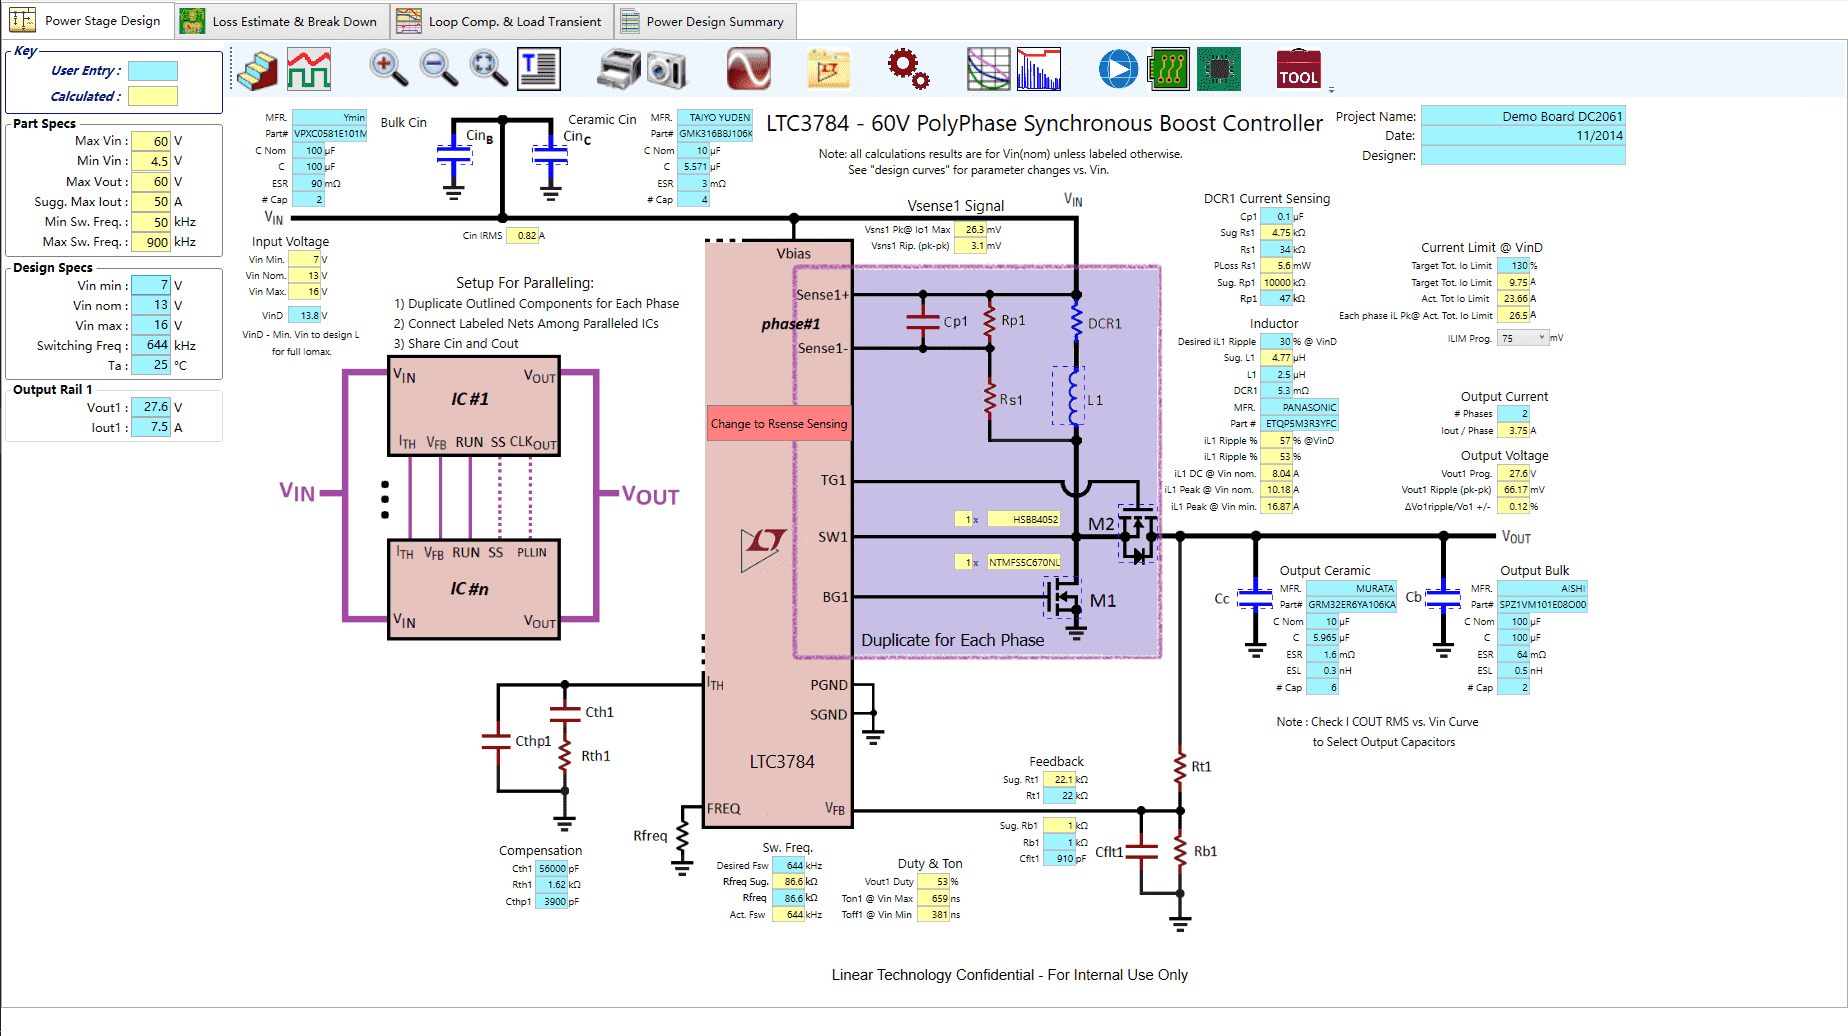
\includegraphics[width=0.5\columnwidth]{figure/设计方案/硬件设计/Boost_LTPowerCAD.png}
    }
    \subfigure[在LTspice中搭建仿真原理图 \label{fig:ltspice_simulation}]{
        \centering
        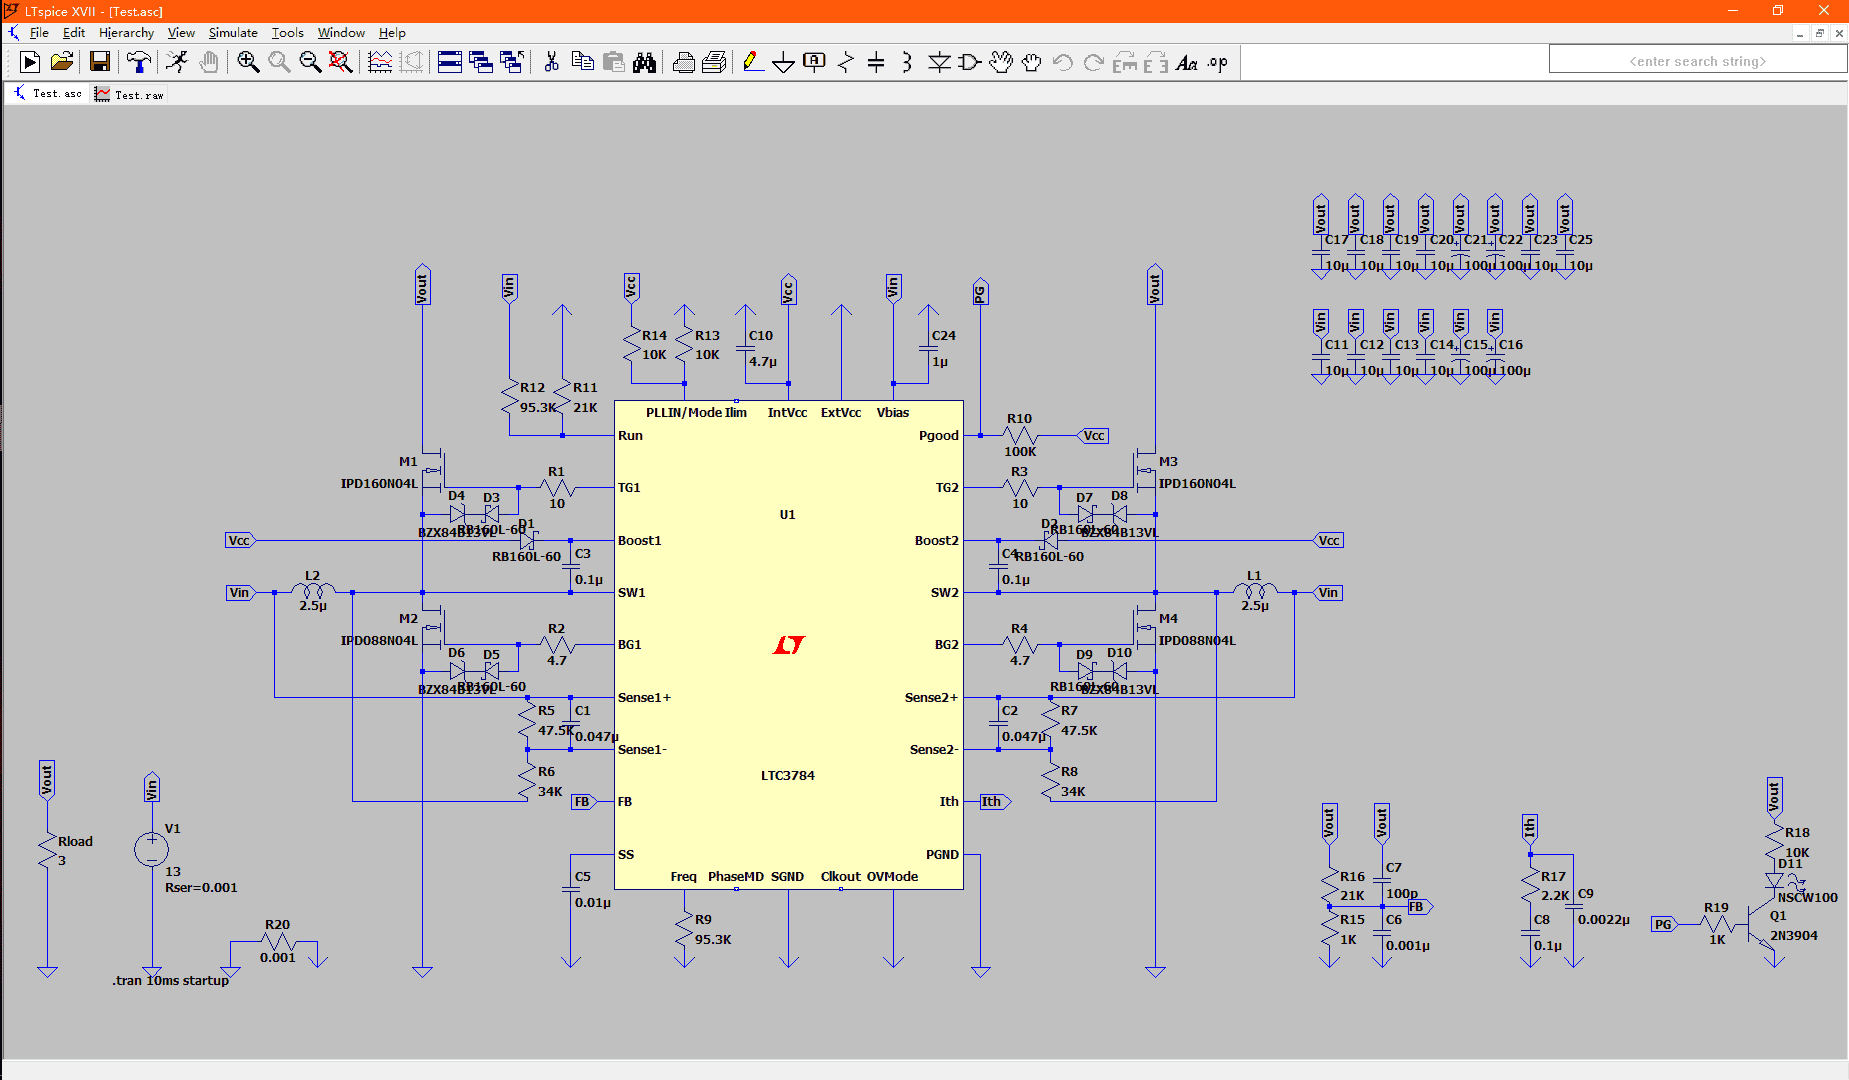
\includegraphics[width=0.45\columnwidth]{figure/设计方案/硬件设计/Boost_LTSPICE.png}
    }
    \caption{部分设计界面展示 \label{fig:boost_design_page}}
\end{figure}

\subsection{发射中心板}
在机器人设计中，IMU模块被放置在了发射机构上，但是IMU模块的供电应隶属于“Gimble（云台）”而非“Ammo-Booster（发射）”，为了方便机器人线路的排布，我们设计了一款自制的中心板，输入供电端子为“MR60”端子，三端分别为Gimble、Ammo-Booster和GND。
自制发射中心板板载了6路CAN接口（GH1.25）、3路发射供电接口（XT30）、2路云台供电接口（XT30）以及IMU专属接口（GH1.25——4Pin），接口全部采用立插，极大的方便了机器人的安装与检修。
\begin{figure}[hbt!]
    \centering
    \subfigure[中心板PCB 3D图\label{fig:中心板PCB 3D图} ]{
        \centering
        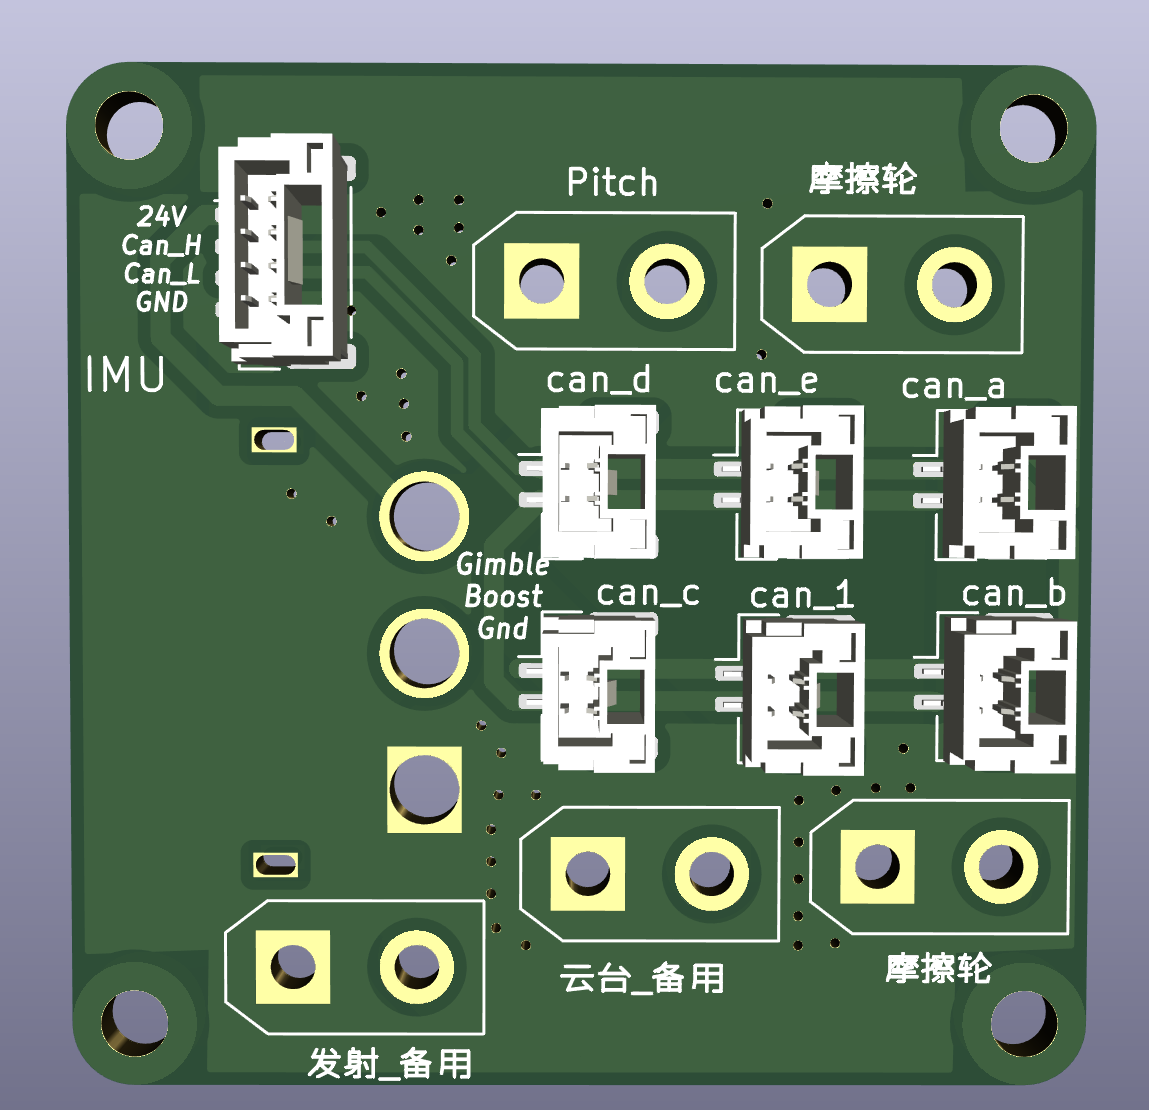
\includegraphics[height=0.4\columnwidth]{figure/设计方案/硬件设计/中心板.png}
    }
    \subfigure[中心板实物图\label{fig:中心板实物}]{
        \centering
        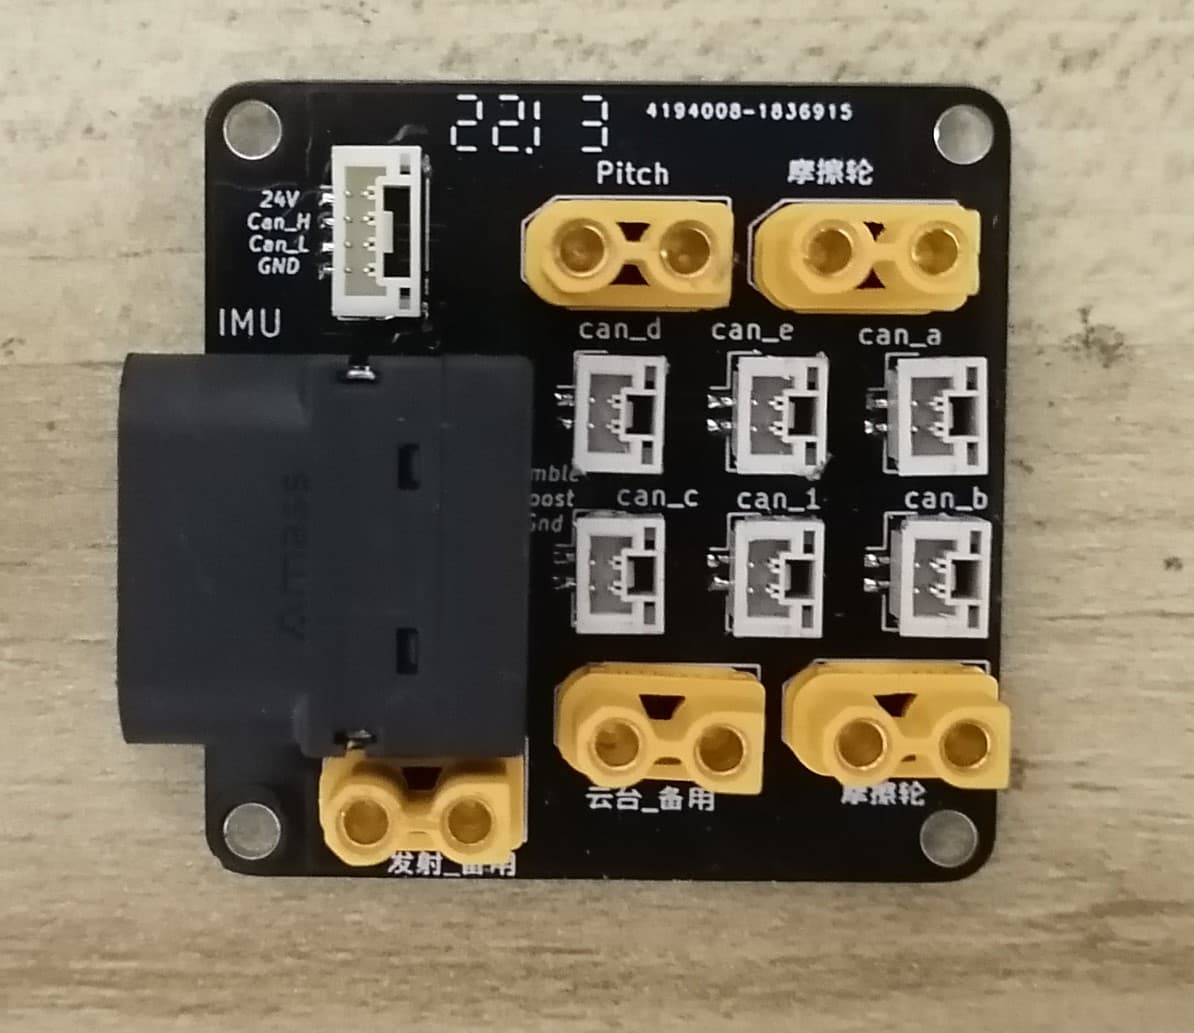
\includegraphics[height=0.4\columnwidth]{figure/设计方案/硬件设计/中心板实物.jpg}
    }
    \caption{自制中心板展示 \label{fig:自制中心板展示}}
\end{figure}

\subsection{NUC降压模块}
由于我们步兵机器人使用的主控是 Intel NUC（以下简称为 NUC），所以需要单独为 NUC 制作一个供电电压为 $\qty{19}{\V}$，供电电流为 $\qty{6.35}{\A}$ 的降压电源。主芯片我们选取LM3150为Buck控制器，LM3150 最高输入电压可达$\qty{42}{\V}$，输出电流可达$\qty{12}{\A}$，满足 NUC 供电需求。另外，LM3150 还工作在 COT（恒定导通时间）模式，具有优异的瞬态响应性能和低压差输出的能力。

最终设计原理图如 \figref {fig:nucpower_设计方案}所示。实
际测量中，在负载电流达到 $\qty{6}{\A}$ 时，NUC 供电电源的效率可以达到$97.8\%$，
模块整体平均温度被控制在 $\qty{50}{\degreeCelsius}$ 以
下，有非常优越的性能表现。

\begin{figure}[hbt!]
    \centering
    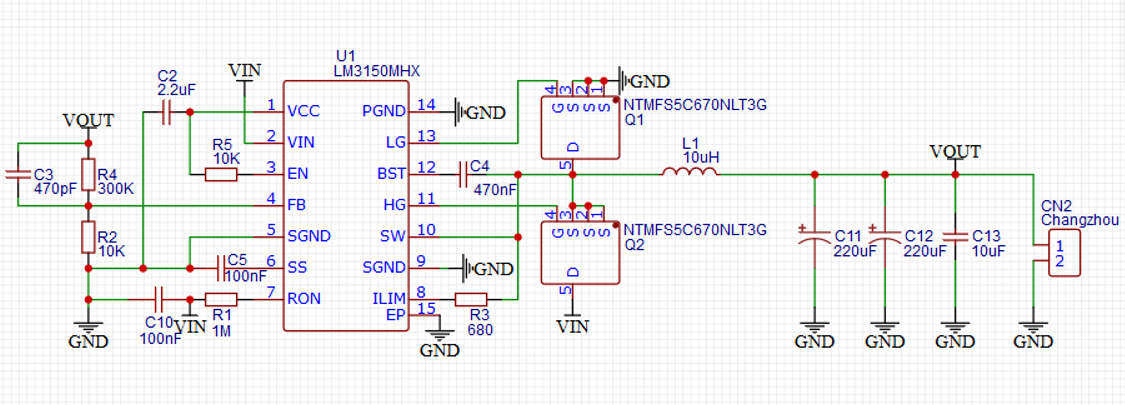
\includegraphics[width=0.9\columnwidth]{figure/设计方案/硬件设计/nucpower.png}
    \caption{LM3150原理图}        
    \label{fig:nucpower_设计方案}
\end{figure}


\subsection{协议转换模块}
为满足不同通信协议的通信，我们设计了多种不同的协议转换模块。在步兵机器人上，我们设计了USB转CAN模块和USB转串口模块，模块主要用于NUC和其它硬件模块之间的通信和控制电机。
\begin{itemize}
    \item USB转CAN部分我们基于 github 的开源方案 candleLight 开发，采用 STM32F072CBT6 作为主控芯片，实现USB转CAN的功能。STM32F072CBT6具有能够同时工作的 USB 全速外设和 CAN 外设，封装为 QFP64，是较为优秀的解决方案。
    \item USB转串口部分主芯片选取CH340E，该芯片是常用的一款USB 总线的转接串口芯片。
\end{itemize}

由于整车需要多路CAN总线来保证电机回传数据包的完整性，我们选取GL850G作为 USB HUB 芯片实现 USB 一拖四的方案，CAN 电平转换芯片采用 MAX3051EKA 芯片， 该芯片使用 $\qty{3.3}{\V}$ 供电且封装为 SOT23-8，为 PCB 小型化提供了基础。同时我们还通过使用施密特触发器来实现上电时序，保证USB设备枚举的顺序在每次上电后都是一致的。

\subsection{惯性测量单元}
为提高机器人姿态获取的精密性、运动控制的准确性，我们使用了六轴惯性测量单元BMI088。该六轴惯性测量单元具有卓越的抗震性能，能保证在冲击下的工作稳定性。为改善惯性测量单元的温飘问题，我们增加了加热电路，通过PID实现对陀螺仪的恒温处理。

相对应的，我们设计了专用于BMI088的控制板。该控制板使用STM32F103C8T6作为主控，通过SPI协议与BMI088通讯，并且集成了一路CAN信号转化电路，能够较便捷地对外通信。
BMI088及其控制板的设计原理图如 \figref {fig:BMI088_设计方案}与 \figref {fig:IMUbase_设计方案}所示。
\begin{figure}[hbt!]
    \centering
    \subfigure[BMI088原理图\label{fig:BMI088_设计方案} ]{
        \centering
        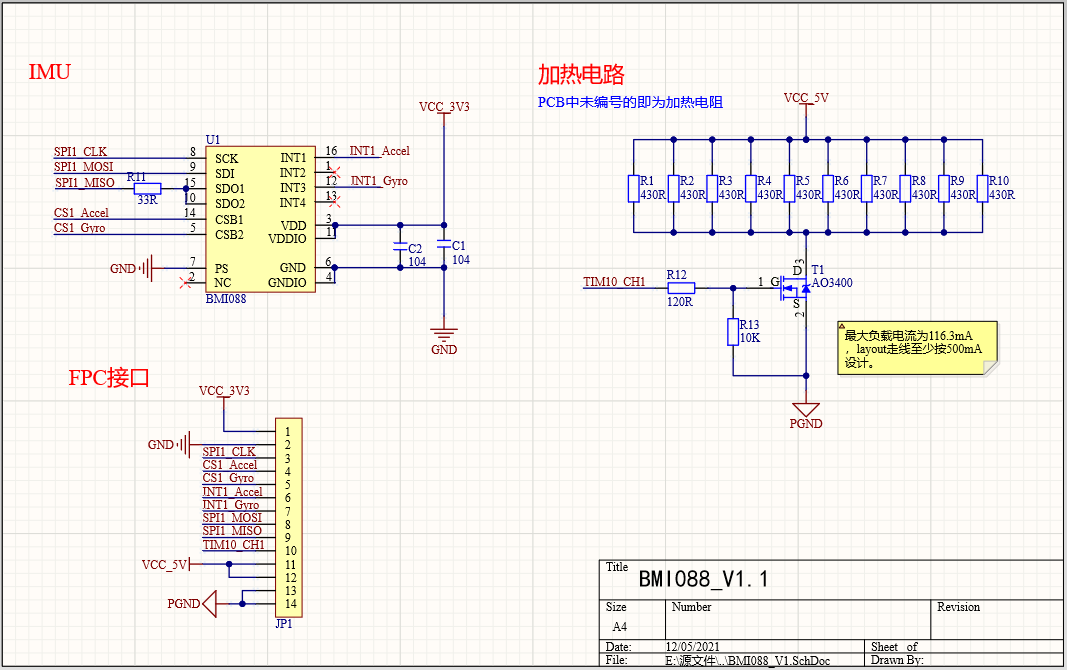
\includegraphics[height=0.4\linewidth]{figure/设计方案/硬件设计/BMI088.png}
    }
    
    \subfigure[IMUbase原理图\label{fig:IMUbase_设计方案}]{
        \centering
        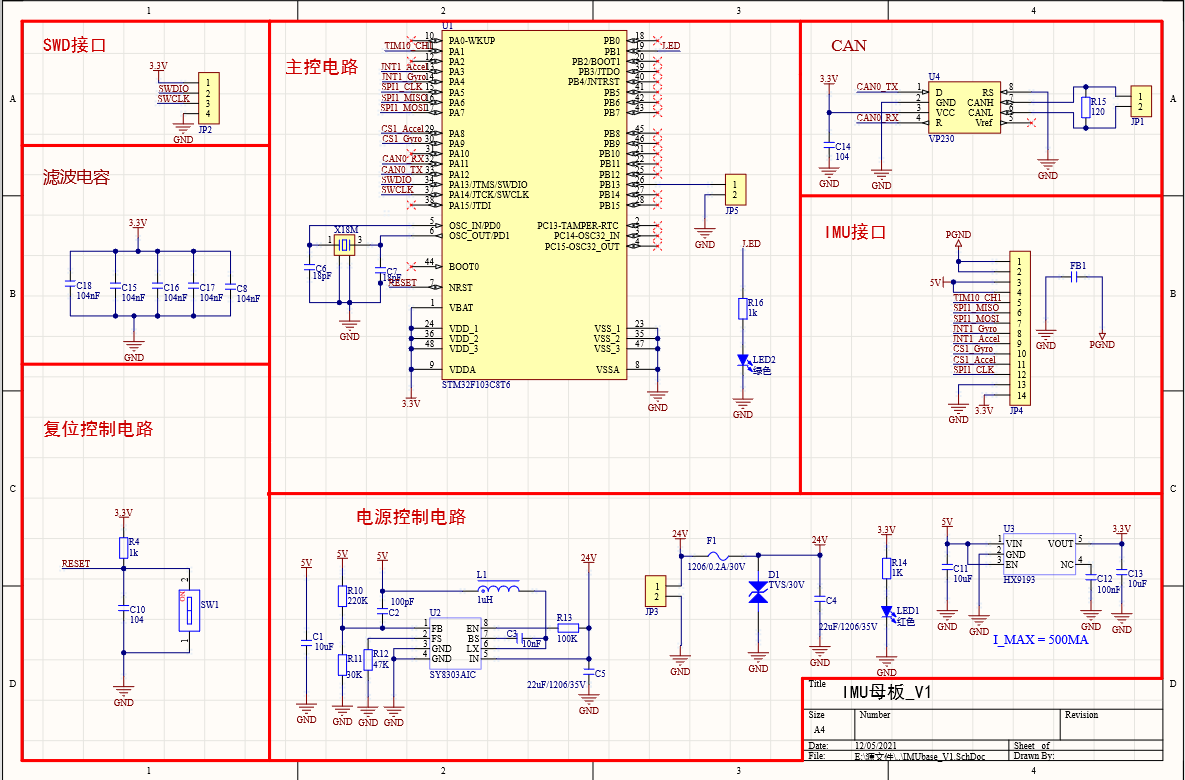
\includegraphics[height=0.4\linewidth]{figure/设计方案/硬件设计/IMUbase.png}
    }
    \caption{IMU模块 \label{fig:IMU模块设计方案}}
\end{figure}

\subsection{荧光充能装置}
比赛中需要使用荧光弹丸，弹丸在经过特定波长紫外光照射充能后，能够发出黄绿色光并显示弹丸飞行轨迹。因此需要设计一款充能装置，产生特定紫外光以进行荧光充能。我们将荧光充能装置分为两个部分：
\begin{itemize}
    \item 紫外光LED灯板。采用封装为2835的390-410nm的紫外灯珠，灯珠发光角度$\ang{120}$，单颗功率$\qty{0.2}{\W}$。我们的设计中采用四串两并的LED灯珠，并使用铝基板以保证足够的散热。
    \item LED恒流驱动板。我们使用BP1360作为恒流驱动，在$\qty{24}{\V}$工作电压下选择$\qty{68}{\mA}$的驱动电流，以此保证紫外光灯板总体功率大于$\qty{1.5}{\W}$。该芯片采用极少的外部元器件，能够快速通过采样电阻设置恒流电流的大小。
\end{itemize}
紫外光LED灯板和恒流驱动板的设计原理图如 \figref {fig:紫外光LED灯板_设计方案}与 \figref {fig:LED恒流驱动板_设计方案}所示。
\begin{figure}[hbt!]
    \centering
    \subfigure[紫外光LED灯板原理图\label{fig:紫外光LED灯板_设计方案} ]{
        \centering
        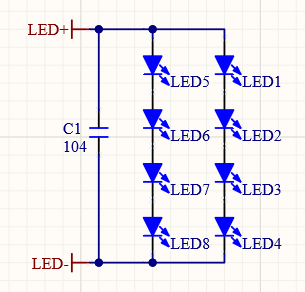
\includegraphics[height=0.3\columnwidth]{figure/设计方案/硬件设计/紫外光LED灯板.png}
    }
    \subfigure[LED恒流驱动板原理图\label{fig:LED恒流驱动板_设计方案}]{
        \centering
        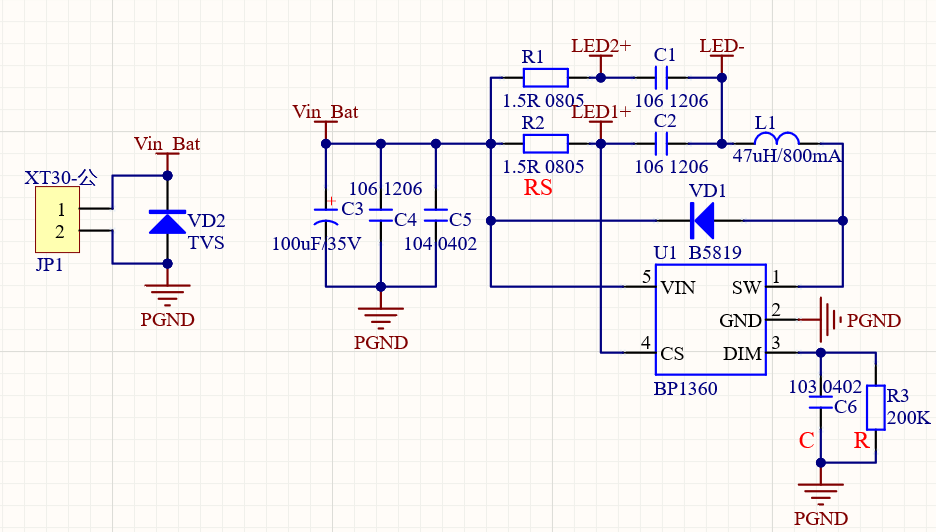
\includegraphics[height=0.3\columnwidth]{figure/设计方案/硬件设计/LED恒流驱动板.png}
    }
    \caption{荧光充能装置 \label{fig:荧光充能装置}}
\end{figure}
\clearpage


